\documentclass[runningheads,a4paper]{llncs}
\usepackage{cite}
\usepackage{graphicx}
\usepackage{listings}
 
%-------------------------------------------------
% Comments/Collaboration
%-------------------------------------------------
\usepackage[dvipsnames]{xcolor}
\usepackage{todonotes}
\newcommand\will[1]{\todo[author=Will,color=Orchid]{#1}}
\newcommand\tim[1]{\todo[author=Tim,color=Apricot]{#1}}
\newcommand\richard[1]{\todo[author=Richard,color=JungleGreen]{#1}}

\authorrunning{Ran Wei, Tim P. Kelly, Richard Hawkins}

\makeatletter
\renewcommand\subsubsection{\@startsection{subsubsection}{3}{\z@}%
	{-18\p@ \@plus -4\p@ \@minus -4\p@}%
	{4\p@ \@plus 2\p@ \@minus 2\p@}%
	{\normalfont\normalsize\bfseries\boldmath
		\rightskip=\z@ \@plus 8em\pretolerance=10000 }}
\renewcommand\paragraph{\@startsection{paragraph}{4}{\z@}%
	{-12\p@ \@plus -4\p@ \@minus -4\p@}%
	{2\p@ \@plus 1\p@ \@minus 1\p@}%
	{\normalfont\normalsize\itshape
		\rightskip=\z@ \@plus 8em\pretolerance=10000 }}
\makeatother

\begin{document}
 
\title{\textbf{Towards A Systematic Approach For Model Based System Assurance}}
\author{Ran Wei \and Tim P. Kelly \and Richard Hawkins}
\institute{University of York, United Kingdom 
\email{\{ran.wei,tim.kelly,richard.hawkins\}@york.ac.uk}
}
\maketitle

\begin{abstract}
Assurance cases are used to demonstrate confidence in properties of interest for a system, e.g. for safety or security. Typically, the task of constructing assurance cases is a lengthy and informal process. In recent years, there has been work to propose model based approaches to promote automation. The Structured Assurance Case Metamodel (SACM) is an OMG specification designed to represent system assurances in machine-readable models, so that a series of model management operations can be 
performed to automate the process of system assurance. However, the adoption of SACM faces challenges as there is a cognitive gap between the syntax/semantics of SACM elements and system assurance practitioners' understanding of SACM.

In this paper, we provide a definitive guide to SACM with examples so that SACM can be better understood. We also discuss the relationship between SACM and the Goal Structuring Notation (GSN) and the interoperability between them. We also propose a systematic approach for model based system assurance using SACM, so that all corresponding models can be bridged together using the facilities provided in SACM.
\end{abstract}


\section{Introduction}
Systems/services used to perform critical functions require justifications that they exhibit necessary properties (i.e. safety and/or security). 
\textit{Assurance case}s provide an explicit means for justifying and assessing confidence in these critical properties. 
In certain industries, typically in the safety-critical domain, it is a regulatory requirement that an assurance case is developed and reviewed as part of the certification process \cite{healthFound}.
An assurance case is a document that facilitates information exchange between various system stakeholders (e.g. between operator and regulator), where the knowledge related to the safety and security of the system is communicated in a clear and defend-able way \cite{hawkins2013assurance}. 

Assurance cases are typically represented either textually - using natural languages; or graphically - using structured graphical notations such as the Goal Structuring Notation (GSN) \cite{kelly2004goal} or Claims-Arguments-Evidence (CAE) \cite{bishop2000methodology}. 
Graphical notations have gain popularity due to their abilities to express clear and well structured argumentations.
A number of tools exist which implement GSN and CAE to produce safety cases \cite{maksimov2018}. 
Some tools adopt Model-Driven Engineering (MDE) to produce models that conform to their own versions of GSN/CAE metamodels \cite{denney2017tool, matsuno2010dependability, netkachova2014tool, larrucea2017supporting, barry2011certware}.

To improve standardisation and interoperability, the Object Management Group (OMG) specified and issued the Structured Assurance Case Metamodel (SACM). 
SACM is developed by the specifiers of existing system assurance approaches (e.g. GSN and CAE), based on the collective knowledge and experiences of safety/security practitioners.
Comparing to existing assurance case approaches, SACM provides additional features such as fine-grained modularity, controlled vocabulary, and argument-evidence traceability. 
Therefore, SACM is more powerful in terms of expressiveness. 
However, neither detailed explanation has been provided in the OMG specification to demonstrate how to use SACM, nor the relationships between existing assurance case approaches (i.e. GSN and CAE) and SACM has been discussed. 
This brings challenges to the adoption of SACM due to the complexity of SACM and the sophistication of its intended usage. 

Model-based system assurance has attracted a significant amount of interests in recent years due to the benefits provided by MDE such as automation and consistency. 
Model-based system assurance is particularly important for concepts such as Open Adaptive Systems (OAS), where open (safety/security critical) systems connect to each other, and adapt to changing contexts at runtime. 

As the principal contributors of SACM and the originators of GSN, in this paper, we provide a detailed explanation of SACM and discuss its relationship with existing system assurance approaches (i.e. GSN and CAE). 
%We first discuss the motivaion of our work. 
%We then provide detailed discussions about the facilities provided by SACM. 
%We demonstrate how SACM can be used to construct an assurance case using examples, and how to maintain the traceability between the argumentation of assurance cases and their supporting evidence/artefacts. 
%We finally discuss briefly tool support for model-based system assurance.
The contributions of this paper are as follows:
\begin{itemize}
	\item A definitive exposition of SACM version 2.0;
	\item A detailed discussion on how to use SACM to create an assurance case model.
	\item GSN and CAE metamodels that are compliant with SACM;
	\item Comprehensive mappings from GSN/CAE to SACM;
\end{itemize}

This paper is organised as follows. 
In Section~\ref{sec:background} and Section~\ref{sec:gsn}, we provide the background and the motivation of our work. 
In Section~\ref{sec:sacm} we provide detailed discussions about the facilities provided by SACM.
In Section~\ref{sec:examples} we provide examples to illustrate the semantics of the elements provided in SACM, and how to use SACM to construct argumentation patterns, and how to integrate assurance cases.
In Section~\ref{sec:mapping}, we discuss the relationship between existing notations and SACM. 
We provide SACM compliant metamodels for GSN and CAE and their mappings to SACM. 
In Section~\ref{sec:toolsupport}, we briefly discuss tool support for model-based system assurance. 
We finally conclude the paper in Section~\ref{sec:conclusion}.



\section{Background and Motivation}
\label{sec:background}

\subsection{Safety Cases}
The concept of assurance cases has been long established in the safety-related domains, where the term \textit{safety case} is normally used. 
For many industries, the development, review and acceptance of a safety case form a key element of regulatory processes. 
This includes the nuclear \cite{hse}, defence \cite{mod2007}, civil aviation \cite{caa2007} and railway \cite{yellowBook2007} industries. 
Safety cases are defined in \cite{kelly2004goal} as follows: \textit{A safety case should communicate a clear, comprehensible and defensible argument that a system is acceptably safe to operate in a particular context}. 

Historically, safety arguments were typically communicated in safety cases through free text. However, there are problems experienced when text is the only medium available for expressing complex arguments. 
One problem of using free text is that the language used in the text can be unclear and poorly structured, there is no guarantee that system engineers would produce safety cases with a clear and well-structured language. 
Also, the capability of expressing cross-references for free text is very limited, multiple cross-references can also disrupt the flow of the main argument. 
Most importantly, the problem with using free text is in ensuring that all stakeholders involved share the same understanding of the argument to development, agree and maintain the safety arguments within the safety case \cite{kelly2004goal}.

To overcome the problems of expressing safety arguments in free text, graphical argumentation notations were developed. 
Graphical argumentation notations are capable of explicitly representing the elements that form a safety argument (i.e. requirements, claims, evidence and context), and the relationships between these elements (i.e. how individual requirements are supported by specific claims, how claims are supported by evidence and the assumed context that is defined for the argument). 
Amongst the graphical notations, the \textit{Goal Structuring Notation} (GSN) \cite{kelly2004goal} has been widely accepted and adopted \cite{chinneck2004turning}. 
The key benefit experienced by companies/organisations adopting GSN is that it improves the comprehension of the safety argument amongst all of the key project stakeholders (e.g. system developers, safety engineers, independent assessors and certification authorities), therefore improving the quality of the debate and discussion amongst the stakeholders and reducing the time taken to reach agreements on the argument approaches being adopted.

Another popular graphical argumentation notation is \textit{Claims-Arguments-Evidence} (CAE) \cite{bishop2000methodology}. 
CAE views assurance cases as a set of \textit{Claim}s supported by \textit{Argument}s, which in turn rely on \textit{Evidence}.
Compared to CAE, 
%GSN provides more granular decomposition of safety arguments into \textit{Goal}s, \textit{Context}s, \textit{Assumption}s, \textit{Justification}s, \textit{Strateg-}ies and \textit{Solution}s. 
GSN supports additional features such as \textit{Module}s, \textit{Contract Modules} and argument templates (GSN Patterns) to promote modularity and re-use.
In this paper, we focus on GSN (and its relationship to SACM) since we are the principal contributors to the standardisation of both GSN and SACM.

A number of graphical assurance case tools have been developed due to the popularity of graphical argumentation notations. 
A recent study \cite{maksimov2018} has looked into and compared assurance case tools that have been developed in the past twenty years (where 32 of them support GSN). 
The majority of the tools do not support model-based approach (i.e. creating model-based graphical assurance cases).
Whilst graphical assurance cases are valuable in communicating the safety and/or security properties of the system, model-based assurance cases enable higher level model management operations to be performed.
%, such as automated validation, model merging and model-to-model transformations. 
%
%However, the claimed support for SACM in fact refer to SACM version 1.0 (released in June, 2015), which was replaced by SACM version 2.0 (released in March, 2018). 

%Whilst the assurance case diagrams produced by the tools are valuable in communicating system assurance argumentations amongst stakeholders, the diagrams are mostly not model-based (except for the ones created by CertWare \cite{barry2011certware} and Astah GSN \cite{larrucea2017supporting}). 
%Thus, automated model management operations (model-to-model transformations, model-to-text transformations, model validations, model mergings, etc.) on such diagrams can not be performed on the diagrams. 

\subsection{Safety Cases and Model Driven Engineering}
Model-Driven Engineering (MDE) is a contemporary software engineering approach. 
In MDE, \textit{model}s are first class artefacts, therefore \textit{driving} the development. 
There are two important aspects in MDE: domain specific modelling and model management. 
Domain specific modelling enables domain experts to capture the concepts in their systems in the form of \textit{metamodel}s, which are then used to create models of their systems (that conform to the defined \textit{metamodel}s). 
Model management enables a variety of operations to be performed on models in an automated manner, which include, but not limited to: Model Validation, Model-to-Model Transformation, Model-to-Text Transformation and Model Merging.
MDE has been proven to improve consistency and productivity significantly due to the automation provided by model management operations \cite{jaaksi2002developing, karna2009evaluating}. 

MDE is particularly beneficial to system assurance.
For example, model validation can be used to check well-formedness of assurance cases (e.g. that a \textit{Strategy} cannot be directly supported by a \textit{Solution}); model-to-text transformation can be used to generate assurance case report; model merging can be used to bind assurance cases, etc. 
A number of assurance case tools adopt MDE, such as AdvoCATE \cite{denney2017tool}, D-Case Editor \cite{matsuno2010dependability}, ASCE \cite{netkachova2014tool}, Astah GSN \cite{larrucea2017supporting}, and CertWare \cite{barry2011certware}. 
However, a common problem with these tools is that they define their own GSN metamodels. 
This is due to the fact that there has not been an standard GSN metamodel (apart from the mappings from GSN to SACM provided on the GSN website\footnote{\url{http://www.goalstructuringnotation.info/}}).
Thus, there may be interoperability problems when one wishes to import GSN models created by other tools to his/her own tool. 
Although the tools mentioned above all claim to support SACM, the support was for SACM version 1.0 (realsed in June, 2015), which was replaced by SACM version 2.0 (released in March, 2018).
Since SACM version 1.0 was also not sufficiently explained (no work has been done in this aspect), there may be cognitive gaps between different tool developers, so that exported SACM models from the tools may differ.
In addition, a considerable amount of changes have been introduced to SACM 2.0, the claimed support for SACM of these tools are out-dated. 

\subsection{Assurance Cases and the Structured Assurance Case Metamodel}
There has been an increasing interest in the use of structured argumentation in other domains, particularly for demonstrating system security \cite{bloomfield2010safety}. 
Such argumentations are typically referred to as \textit{security cases}. 
The similarities between safety and security cases have been highlighted in \cite{lautieri2005safsec}. 
Therefore, the term \textit{assurance case} is a broader definition: \textit{An assurance case should communicate a clear, comprehensible and defensible argument that a system/service is acceptably safe and/or secure to operate in a particular context.} 

To promote standardisation and interoperability, the Object Management Group (OMG) specified and issued the \textit{Structured Assurance Case Metamodel} \cite{sacm}. 
SACM is developed by the developers of system assurance approaches (e.g. GSN and CAE), based on the collective knowledge and experiences of safety and/or security practitioners over the period of two decades. 
Because of this, features that are not supported by GSN and CAE have been evaluated and included in SACM. 
A selection of such features are summarised in Table~\ref{tab:feature} (with an indicative but non-exhaustive list of works that motivate the features).

\begin{table}[]
	\centering
	\begin{tabular}{|l|l|}
		\hline
		\textbf{Feature}               & \multicolumn{1}{c|}{\textbf{Motivated By}}                        \\ \hline
		F1. Modularity            & \multicolumn{1}{c|}{\cite{despotou2008investigating}} \\ \hline
		F2. Controlled Vocabulary &\multicolumn{1}{c|}{\cite{luo2015safety, attwood2014use}}                  \\ \hline
		F3. Traceability from Evidence to Artifact &\multicolumn{1}{c|}{\cite{taguchi2014linking}}                  \\ \hline
		F4. Automated Assurance Case Instantiation &\multicolumn{1}{c|}{\cite{hawkins2015need, hawkins2015weaving}}                  \\ \hline
		F5. Describing the Level of Trust in Arguments &\multicolumn{1}{c|}{\cite{fenn2005putting}}                  \\ \hline
		F6. Counter-Arguments in Assurance Cases &\multicolumn{1}{c|}{\cite{armstrong2004deconstruction}}                  \\ \hline
		F7. Multiple Language Support &\multicolumn{1}{c|}{\cite{denney2013formal}}                  \\ \hline
	\end{tabular}
	\caption{Features added to SACM}
	\label{tab:feature}
\end{table}

\textbf{Modularity (F1)}. It is important to promote modularity for assurance cases, so that system safety/security can be argued on a component basis (instead of having a huge assurance case diagram) \cite{despotou2008investigating}. 
Modularity is supported by GSN, however, in SACM modularity is more granular due to the fact that the users of SACM are able to create not only argument packages, but also terminology packages, artifact packages and assurance case package.

\textbf{Controlled Vocabulary (F2)}. Various studies have identified the importance of controlled vocabulary used in system assurance arguments \cite{luo2015safety, attwood2014use}. 
In SACM, the users are able to create controlled vocabulary (which can relay to actual model/model elements that define the vocabulary) and refer to them in the assurance argument. 

\textbf{Traceability from Evidence to Artifact (F3)}. In GSN and CAE, evidence in assurance cases are described using natural language, there is no built-in facility that enables the traceability from evidence to the actual artifact. 
Existing work achieves traceability through the use of an external metamodel \cite{taguchi2014linking}.
In SACM, traceability is naturally supported, which will be explained in Section~\ref{sec:sacm}.

\textbf{Automated Assurance Case Instantiation (F4)}. Assurance case templates are useful in capturing good practice in system assurance for re-use.
GSN provides the notion of \textit{GSN patterns}, which enables the users to create abstract safety cases (templates), and then \textit{instantiate} the patterns based on actual system information to create concrete safety cases. 
In~\cite{hawkins2015need} and ~\cite{hawkins2015weaving}, a model based automated pattern instantiation approach is discussed and presented. 
This approach uses a intermediate \textit{weaving model} to link GSN patterns with system models. 
In SACM, automated instantiation can be achieved without the introduction of intermediate models.

\textbf{Describing the Level of Trust in Arguments (F5)}. It is important to argue the trustworthiness of arguments made in an assurance case (F5), motivated in~\cite{fenn2005putting}. 
In GSN and CAE, there is no explicit means to express the level of trust in an argument. 
However, in SACM, there is a facility specifically designed to argue the trustworthiness of an argument.

\textbf{Counter-Arguments in Assurance Cases (F6)}. Sometimes, it is also important to present counter arguments in an assurance case~\cite{armstrong2004deconstruction}.
However, in GSN and CAE there is no specific means to express counter arguments. 
In SACM, an argument can be declared as \textit{counter}, to declare a reversal argument.

\textbf{Multiple Language Support (F7)}. Multiple language support seems trivial in assurance cases created using GSN and CAE.
However, when creating SACM version 2.0 we have realised that the importance of multiple language support not only lies in the means to describe arguments in multiple natural languages, but also lies in the means to describe arguments in formal languages \cite{denney2013formal}.
Arguments described using formal language enable the possibility of automated reasoning of system safety, which is particularly important in the context of runtime model-based system assurance.

As principal contributors of SACM and the originators of GSN, we can conclude that SACM is more powerful than GSN and CAE in terms of expressiveness.
However, in the SACM specification there is limited information on the intended usage of SACM. 
In order to exploit SACM's full potential, and to promote the adoption of SACM, it is necessary to explain SACM in detail so that safety and security engineers can fully use SACM to achieve higher level goals (e.g. automated model validation to check either well-formedness or runtime safety certification). 

In the current state of practice, graphical notations such as GSN remain the most popular approach for system assurance. 
SACM is designed to support GSN, but the OMG specification does not provide a mapping between GSN elements and SACM elements. 
This is due to the fact there has not been a SACM aligned GSN metamodel. 
Thus, in this paper we provide a GSN metamodel which aligns to SACM. 
In addition, there is also a need to translate from GSN to SACM. 
First of all, the OMG has not defined a concrete syntax (i.e. graphical notation) for SACM elements, which makes creating SACM models a tedious and error-prone process. 
Thus, to make the transition from GSN to SACM, it is good practice to use GSN notations to construct arguments and then transform to SACM using model-to-model transformation. 
Secondly, since GSN has been widely adopted in industry, practitioners can convert their legacy diagrams into GSN models, and then transform to SACM to enable model-based system assurance. 
Due to the reasons above, in this paper, we will also provide a mapping (model-to-model transformation) from GSN to SACM.

\subsection{Model-Based System Assurance and Cyber-Physical Systems}
The physical and digital worlds are gradually merging into a largely connected globe. 
This is backed by the emergence of concepts such as Cyber-Physical Systems (CPS).
Openness and adaptivity are core properties of CPS as constituent systems dynamically connect to each other and have to adapt to a changing context at runtime \cite{trapp2013safety}.
CPS harbours the potential for vast economic and societal impact in domains such as automotive, health care, and home automation due to their open and adaptive nature \cite{wei2017deis}.
The majority of application domains of CPS are safety-critical, such as car2car scenarios and collaborative autonomous mobile systems.
If these systems fail, they may cause harm and lead to temporary collapse of important infrastructures, with potential catastrophic consequences for industry and society.
Therefore, it is imperative to ensure the dependability of CPS in order to realise their full potential. 
However, the open and adaptive nautre of CPS poses significant challenges to assuring such systems, as it is nearly impossible to anticipate the concrete CPS structure, its capabilities and the environmental context sufficiently at design time.

Therefore, existing design time system assurance activities are inappropriate to enable dynamic system assurance for CPS at runtime. 
In \cite{trapp2013safety}, the authors identify the importance of system assurance at runtime for CPS and propose the idea of Models@Runtime, in the sense that system assurance information is exchanged when CPSs interconnect with each other to reason about the dependability of the to-be-formed system of systems.

We envision that SACM is the best candidate for AssuranceCase@Runtime in this context, this is backed by the fact that SACM is used in the DEIS project \cite{wei2017deis} as a backbone for its Open Dependability Exchange metamodel (ODE), to ensure the dependability of CPS. 


%SACM also provides multi-language support, in the sense that argumentations can be expressed using computer languages, which is the premise for automated argument reasoning. This is particularly beneficial for CPSs.
%
Therefore, model-based assurance cases are more than `nice diagrams', they are important artefacts which can be used at design time for system integration, as well as at runtime for automated reasoning when runtime assurance is needed for open adaptive systems such as CPS. 

\subsection{Summarised Motivations}
The motivations of our work can be summarised as follows. 
\begin{itemize}
	\item \textbf{Heterogeneous GSN metamodels and misalignment to SACM}.
	Multiple GSN metamodels, where the differences even indicate a different semantical understanding of GSN. 
	
	They often fail to correctly capture the differences between abstract and concrete syntax of GSN. (Metamodel often dictated by concrete syntax of GSN rather than the deep understanding of the semantics of the metamodel).
	
	\item At present in the assurance community, there are two well established notations GSN and CAE. Sometimes false distinctions are made between these notations. E.g. Wrong-footed by the nomenclature, the equivalence of Claim and Goal is not always acknowledged. 
	
	 Graphical notations such as GSN and CAE are the most popular means to create system assurance cases.
	Although a number of model-based assurance case tools exist, they implement their own version of GSN, their mappings from GSN to SACM version 1.0 are not unanimous due to the fact that SACM version 1.0 was not sufficiently explained. 
	In addition, due to the release of SACM version 2.0, the claimed supports for SACM of existing model based GSN/CAE tools become out-dated.
	\item \textbf{Importance of SACM and its application in open adaptive system assurance}. SACM provides more features than GSN/CAE, which makes it more powerful in terms of expressiveness. 
	SACM is fundamental to runtime system assurance, which is the key for open adaptive systems such as Cyber-Physical Systems.
	\item \textbf{Insufficient explanation of SACM}. SACM has been developed over the period of 10 years, and is the result of significant deliberation and consultation. As a consequence, there are many use cases behind the features (known to the authors of this paper as principal authors of the SACM standard) that are present that may not be apparent to users on first inspection.
	E.g. to support existing concepts such as modularity, patterns, and meta argumentation. 
	SACM and the relationship between GSN/CAE and SACM are not sufficiently explained, which hinders its adoption. 
\end{itemize}


\section{Structured Assurance Case Metamodel}

\section{Structured Assurance Case Metamodel and the Goal Structuring Notation}

\begin{figure}
	\centering
	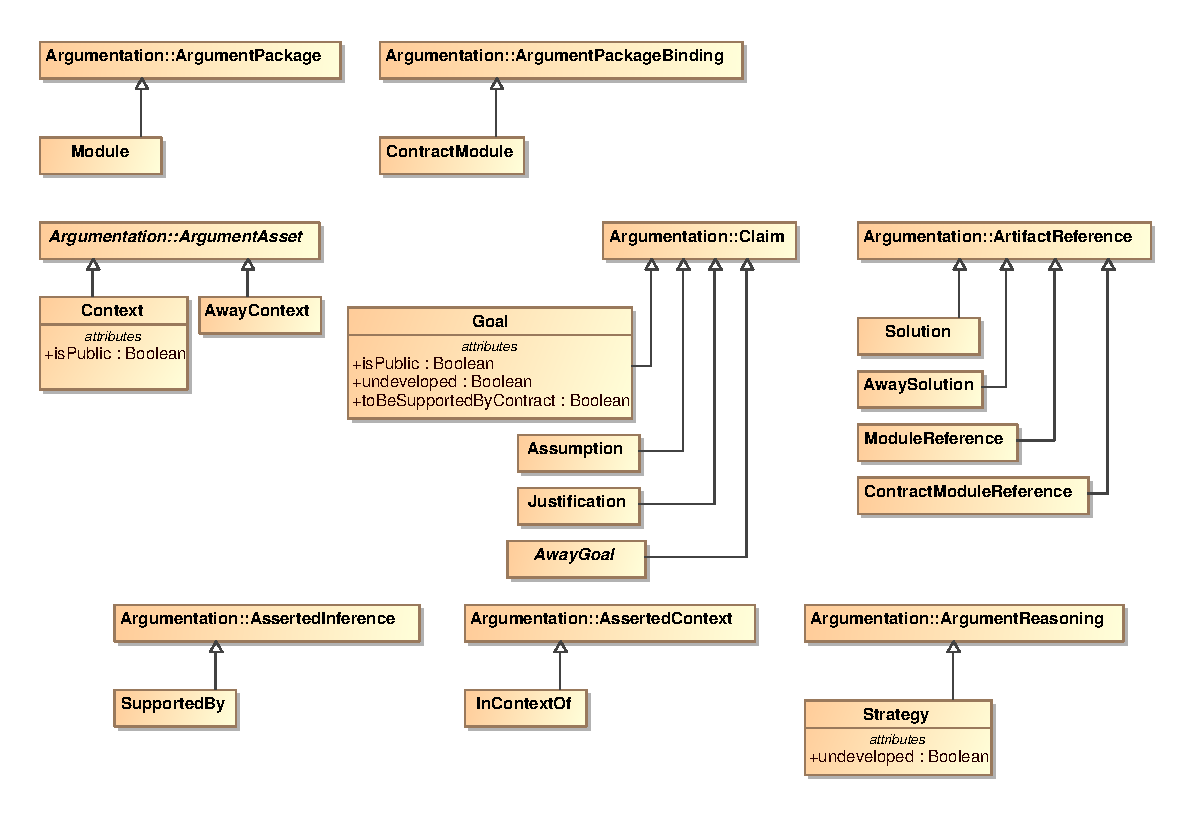
\includegraphics[width=1\linewidth]{GSNMetamodel.eps}
	\caption{An \textbf{asCited} \textit{Claim}.}
	\label{fig:asCitedClaim}
\end{figure}

\section{Running example: a systematic approach}

\section{Tool Support and Related Work}

\section{Conclusion}

Safety Case Construction
and Reuse using Patterns

\noindent\textbf{Acknowledgements}
This work is supported by the European Union'’s Horizon 2020 research and innovation programme through the DEIS project (grant agreement No 732242). 

\bibliographystyle{unsrt} 
\bibliography{references}  

\end{document}
